\chapter{Methodology} \label{cp:methodology}

This chapter outlines the wind tunnel testing procedures, model construction, and data analysis methods used to evaluate the aerodynamic performance of our aircraft design. Key findings from these tests will inform our final design decisions and validate our computational fluid dynamics (CFD) simulations.
% Briefly introduce the topic/purpose of this chapter, what information can be found in this chapter, and the key findings.

\section{Wind Tunnel Testing}

Wind tunnel testing is a critical part of the design of the Banshee, allowing the team to measure the forces and moments acting on a scaled wing model of the aircraft under controlled conditions. The process helps validate CFD simulations and provides real performance data.
% Describe the purpose of wind tunnel testing generally.

\subsection{Wing Testing}

Our wing testing procedure has the following steps:

\begin{enumerate}
    \item Mount the wing model securely to the wind tunnel stand using the provided wood plate (5.5 in x 2.5 in x 0.75 in) with 3.5 in center-to-center holes.
    \item Set the initial AoA to -2° and zero the force/moment transducers with the tunnel off.
    \item Run the wind tunnel at 22.8 MPH, 30 MPH, 35 MPH, and 40 MPH.
    \item Record data output, including $F_x$, $F_y$, $F_z$, $M_x$, $M_y$, and $M_z$ in lb and lb-in.
    \item Increase the AoA in 1° to 2° increments up to stall, repeating steps 1-4 for each angle.
\end{enumerate}

For CFD analysis, we created simulations that match our physical model conditions to enable direct comparisons between experimental and computational results.
The CAD model of the manufactured wing was used to perform aerodynamic analysis using StarCCM+ at various AoAs and at the same speeds as that used for the wind tunnel

% Describe the conditions, apparatus, and procedure for testing the performance of the wind tunnel wing model. Also describe the setup for CFD analysis.

\newpage

\subsection{Motor and Propeller Testing}

Motor and propeller testing will focus on evaluating thrust output and power consumption:

\begin{enumerate}
    \item Conduct static test to measure thrust and current draw at various RPM settings.
    \item Perform dynamic tests simulating cruise conditions to assess propulsion system efficiency.
    \item Use the collected data to estimate flight time in cruise conditions.
\end{enumerate}

We will compare our experimental results with MotoCalc predictions, focusing on thrust output and electrical power consumption rather than direct RPM comparisons.

% Describe the conditions, apparatus, and procedure for testing the performance of the motors and propellers.

\begin{figure}[htpb]
    \centering
    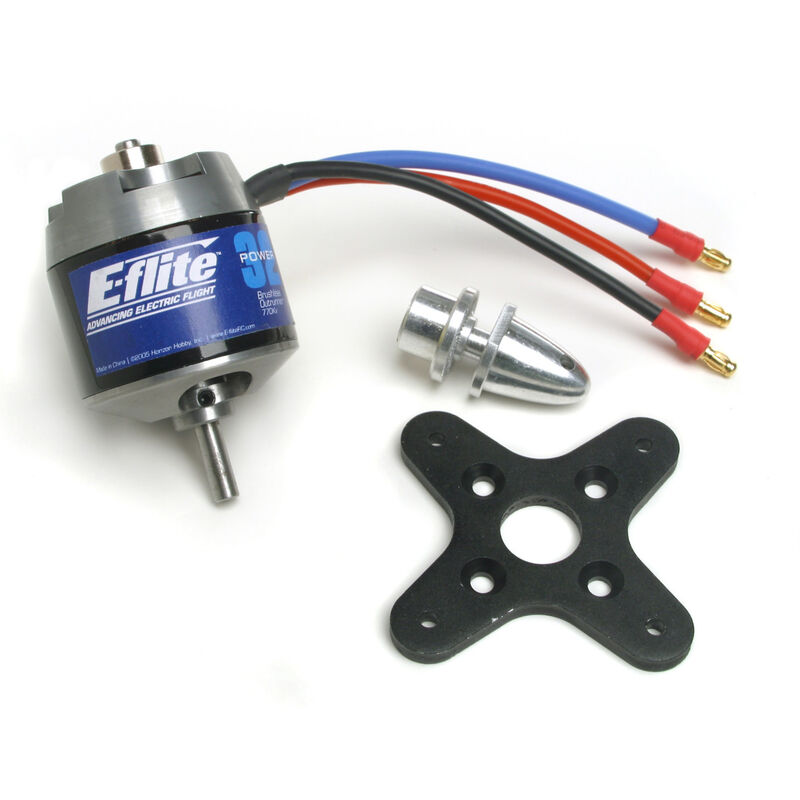
\includegraphics[width=0.88\linewidth]{figures/propulsion_data/eflitepower32.jpg}
    \caption{E-Flite Power 32 Brushless Outrunner Motor.}
    \label{fig:eflitepower32}
\end{figure}

\begin{figure}[htpb]
    \centering
    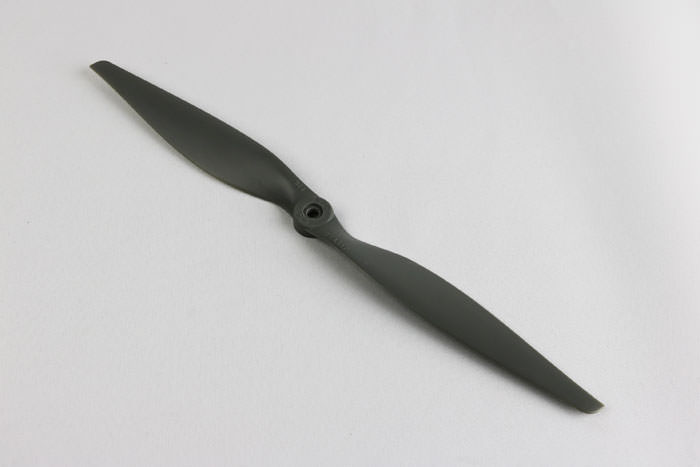
\includegraphics[width=0.88\linewidth]{figures/propulsion_data/apc13x4_5ep.jpg}
    \caption{APC 13x4.5EP Propeller.}
    \label{fig:apc13x4_5ep}
\end{figure}

% \begin{figure}[htpb]
%     \centering
%     \includegraphics[width=0.88\linewidth]{}
%     \caption[}
%     \label{fig:}
% \end{figure}

\newpage

The propulsion system tested consisted of an E-Flite Power 32 motor and an APC 13x4.5E propeller, connected to a power system that simulates a battery with 4 cells in series. The motor and propeller assembly was then mounted in a stand inside the wind tunnel, as seen in \autoref{fig:motor_testing_setup}. Sensors measured acceleration, torque, thrust, voltage, current, rotations per minute, electrical power, mechanical power, motor efficiency, propeller mechanical efficiency, overall efficiency, and vibration. For our purposes, we focused on the thrust and electrical power outputs.

\begin{figure}[htpb]
    \centering
    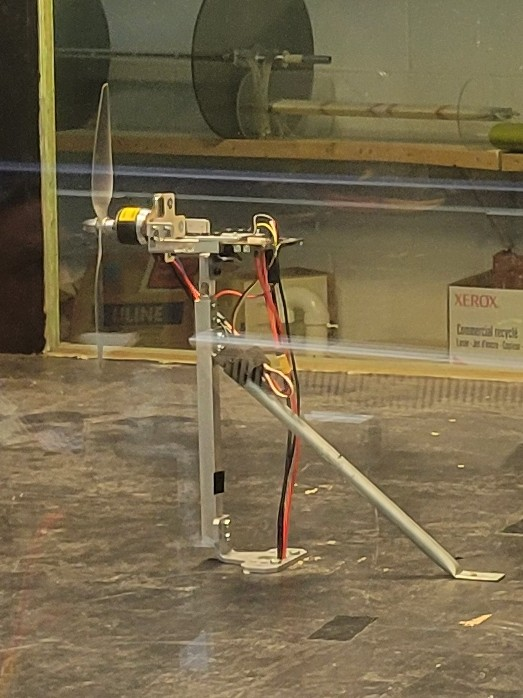
\includegraphics[width=0.88\linewidth]{figures/propulsion_data/motor_testing_setup.jpg}
    \caption{Motor and propeller assembly ready for wind tunnel testing.}
    \label{fig:motor_testing_setup}
\end{figure}

Data was collected at five different wind tunnel speed configurations: static (0 MPH), 22.8 MPH, 30 MPH, 35 MPH (our cruise speed), and 40 MPH.

\newpage

\section{Wind Tunnel Model and Construction}


Our wind tunnel model, shown in \autoref{fig:main_cad}, consists of a 42.5" long foam section representing half the length of our prototype's main wing. Key features of the model include:

\begin{itemize}
    \item Longitudinal reinforcement using 3/8" and 5/8" carbon fiber spars, mirroring the prototype design.
    \item A 3D-printed attachment block housed in a pocket at the wing's bottom, securing the carbon fiber spars.
    \item A wooden adapter plate epoxied to the 3D-printed block, providing attachment to the load sensor and establishing a 0° AoA reference.
\end{itemize}

\begin{figure}[htpb]
    \centering
    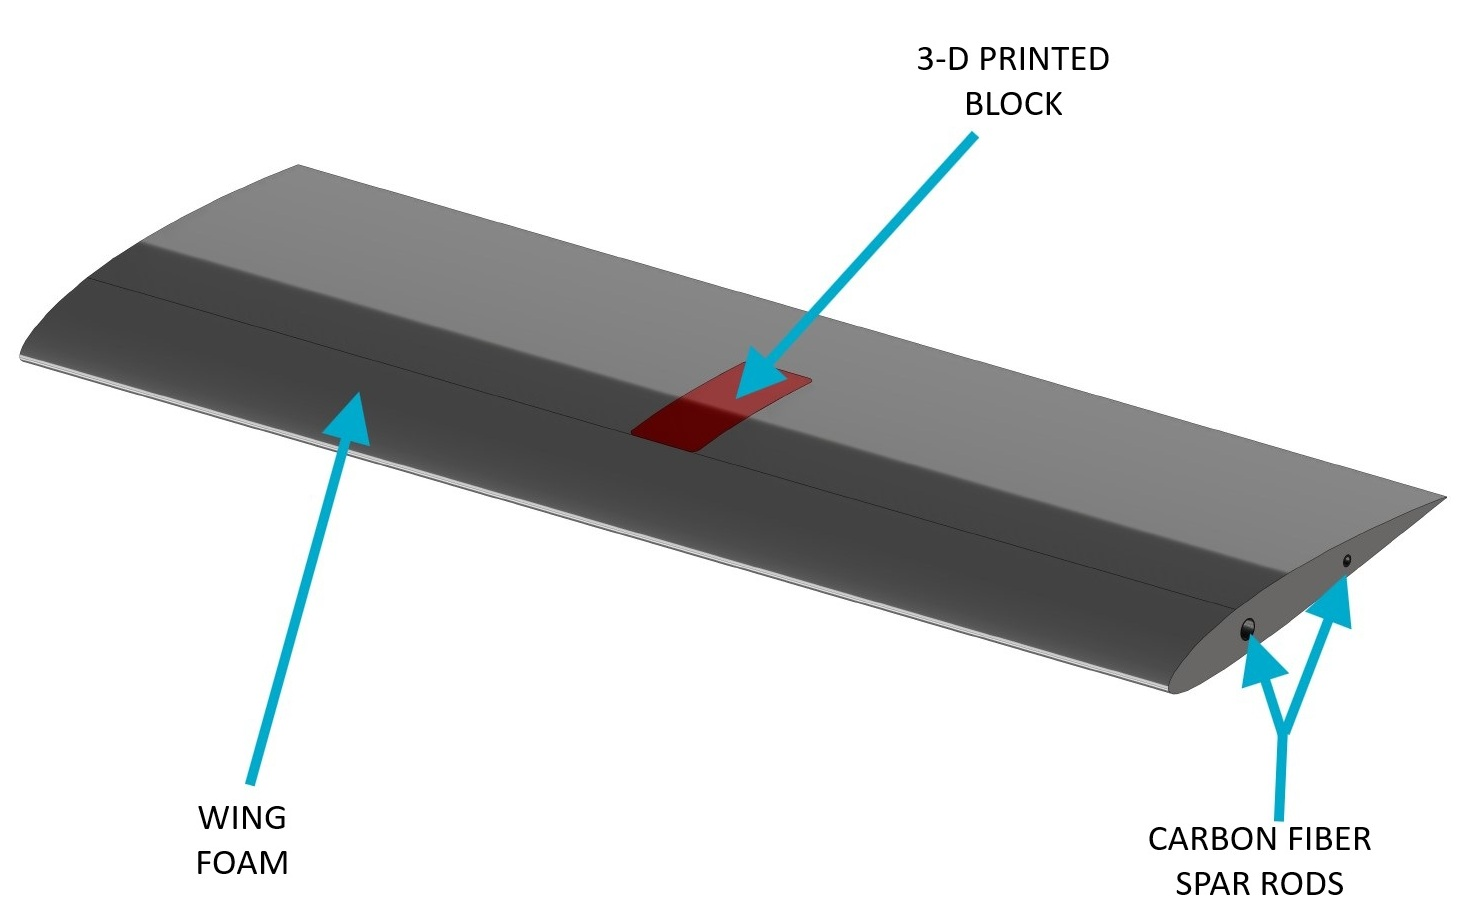
\includegraphics[width=0.88\linewidth]{figures/cad/TestWing_page-0001.jpg}
    \caption[Isometric View of the Wind Tunnel Model]{An isometric view of the wind tunnel model.}
    \label{fig:main_cad}
\end{figure}

\newpage

The wind tunnel model is designed with a focus on stiffness and strength to withstand all wind tunnel tests. Its construction ensures that it accurately represents the aerodynamic characteristics of our prototype, as both have the same chord length, as shown in \autoref{fig:comp_cad}.


\begin{figure}[htpb]
    \centering
    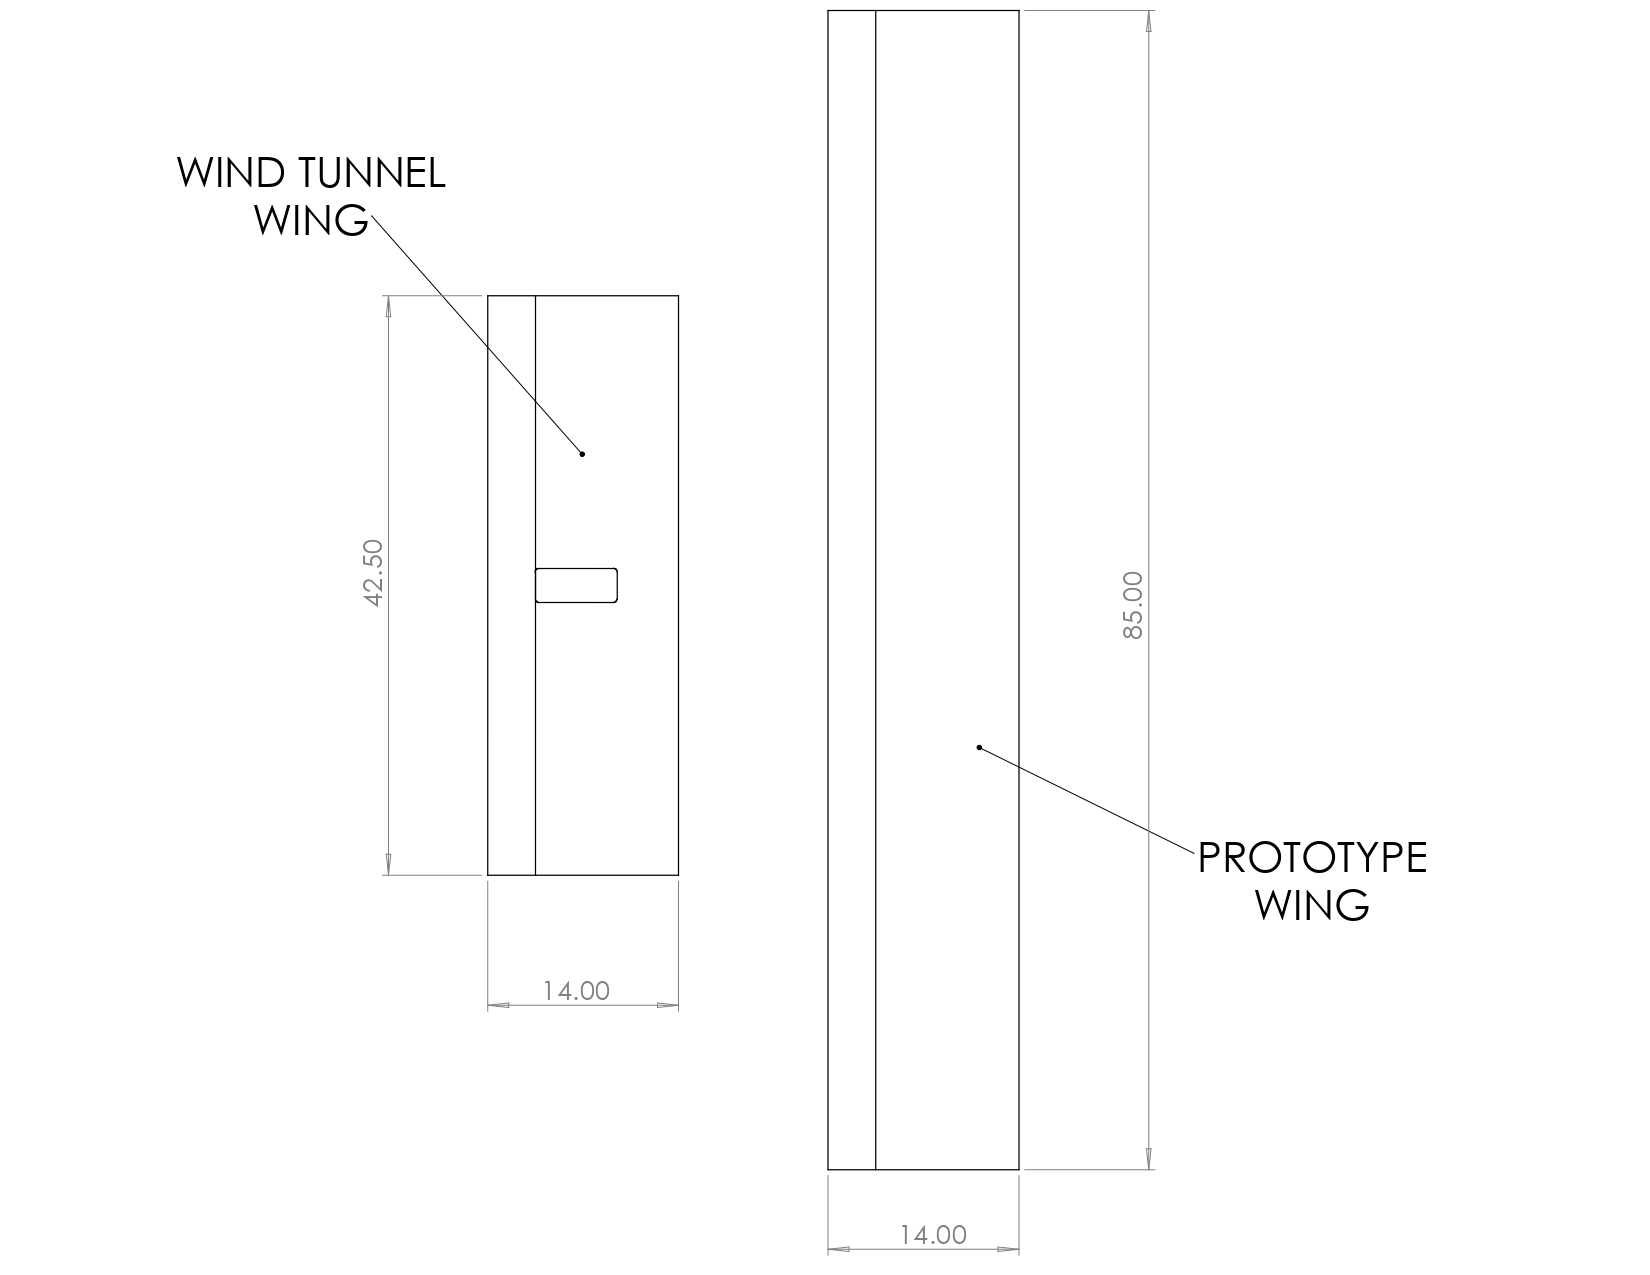
\includegraphics[width=\linewidth]{figures/cad/Wing Comparison_page-0001.jpg}
    \caption[Top View of Wind Tunnel Wing and Prototype Wing]{A top view of the wind tunnel and prototype wings. All dimensions shown are in inches.}
    \label{fig:comp_cad}
\end{figure}

% Describe the design, key dimensions, and construction of the wind tunnel model.
